\chapter{Multi-agent refinement quantified doxastic logic}\label{kd45}

In this chapter we provide an axiomatisation of the multi-agent refinement
quantified doxastic logic. The axiomatisation for the doxastic variant differs
from the modal variant due to the interpretation of the refinement operator.

\section{Technical preliminaries}

In Chapter~\ref{single} we gave an axiomatisation of the single-agent variant of
the refinement quantified doxastic logic. This axiomatisation relied on a
prenex normal form that restricted formulae by prohibiting nested modalities.
The prenex normal form simplified the axiomatisation and proof of soundness by
avoiding complications that would arise due to the transitive and Euclidean
properties of \classKD{} models when nested modalities are present.

For the axiomatisation of the multi-agent variant, we introduce a disjunctive
normal form that serves the same purpose as the prenex normal form served for
the single-agent variant. The disjunctive normal form is a generalisation of the
prenex normal form to multi-agent logics. In multi-agent doxastic logic, it is
not possible to write every formula without using nested modalities; for
example, a formula involving multiple agents, such as $\knows_a \knows_b p$
cannot be simplified any further. Rather, our disjunctive normal form prohibits
modalities of the same agent from being nested directly within one another,
without a modality belonging to another agent appearing inbetween. For example,
$\knows_a \knows_b \suspects_a p$ is allowed, whereas $\knows_a \suspects_a p$ is
not. This allows us to avoid the same complications due to transitivity and
Euclideaness that the prenex normal form allowed us to avoid.

Similar to the prenex normal form used in the single-agent case, we will define
our disjunctive normal form in terms of basic modal operators first, and then
provide another form which is in terms of the cover operator. We will also show
a property of these formulae which we rely on for our soundness proof.

\begin{definition}[Disjunctive normal form]
A formula in $a$-disjunctive normal form is defined by the following abstract syntax:
\begin{eqnarray*}
\alpha &::=& \delta \bnfalt \alpha \lor \alpha\\
\delta &::=& \pi \bnfalt \knows_b \gamma_b \bnfalt \suspects_b \gamma_b \bnfalt
\delta \land \delta\\
\end{eqnarray*}
where $\pi$ stands for a propositional formula, $b \in A - \{a\}$, and
$\gamma_b$ stands for a formula in $b$-disjunctive normal form.

A formula in disjunctive normal form is defined by the following abstract syntax:
\begin{eqnarray*}
\alpha &::=& \delta \bnfalt \alpha \lor \alpha\\
\delta &::=& \pi \bnfalt \knows_a \gamma_a \bnfalt \suspects_a \gamma_a \bnfalt
\delta \land \delta\\
\end{eqnarray*}
where $\pi$ stands for a propositional formula, $a \in A$, and $\gamma_a$
stands for a formula in $a$-disjunctive normal form.
\end{definition}

We will now show that every formula of \lang{} is equivalent to a formula in
disjunctive normal form, under the semantics of doxastic logic.

\begin{lemma}\label{kd45-dnf-equivalences}
We have the following equivalences in \logicKD{}:
\begin{eqnarray*}
\knows_a (\pi \lor (\alpha \land \knows_a \beta)) &\iff& (\knows_a (\pi \lor \alpha)
\land \knows_a \beta) \lor (\knows_a \pi \land \neg \knows_a \beta)\\
\knows_a (\pi \lor (\alpha \land \suspects_a \beta)) &\iff& (\knows_a (\pi \lor \alpha)
\land \suspects_a \beta) \lor (\knows_a \pi \land \neg \suspects_a \beta)
\end{eqnarray*}
\end{lemma}

This is proven by Meyer and van der Hoek~\cite{meyer2004epistemic} for the
single-agent epistemic logic, however the same proof also applies to \logicKD{}.

Meyer and van der Hoek remarked that the only use of the reflexivity axiom of
\logicS{}, {\bf T}, in the proof, is in the form of the theorems $\proves \knows
\knows \phi \implies \knows \phi$, and $\proves \knows \neg \knows \phi \implies
\neg \knows \phi$. Therefore the proof holds for any logic which replaces {\bf
T} with axioms entailing both of these properties. Both of these properties are
obviously valid in \logicKD{}, and therefore the proof by Meyer and van der
Hoek~\cite{meyer2004epistemic} applies to this result.

\begin{lemma}\label{kd45-dnf}
Every formula of \lang{} is equivalent to a formula in disjunctive normal form,
under the semantics of \logicKD{}.
\end{lemma}

\begin{proof}
We use a proof similar to the proof for prenex normal form, given by Meyer and
van der Hoek~\cite{meyer2004epistemic}.

Let $\alpha \in \lang$. Without loss of generality, by Lemma~\ref{k-nnf}, we may
assume that $\alpha$ is in negation normal form. We prove by induction over the
structure of $\alpha$ that $\alpha$ is equivalent to a formula in disjunctive
normal form. The induction hypothesis is that every strict subformula of
$\alpha$ has an equivalent in disjunctive normal form.

The proof is similar to the proof for Lemma~\ref{k-dnf}, except for the cases
where $\alpha = \knows_a \phi$, $\alpha = \suspects_a \phi$ and $\alpha \phi
\lor \psi$.

Suppose that $\alpha = \knows_a \phi$. By the induction hypothesis, there is a
formula $\phi'$ in disjunctive normal form that is equivalent to $\phi$. Suppose
that $\phi'$ is not in $a$-disjunctive normal form (otherwise we are done). Then
$\phi'$ contains some conjunct of the form $\knows_a \beta$ or $\suspects_a
\beta$. Suppose that we have a conjunct of the form $\knows_a \beta$. Then we
can rewrite $\phi'$ as $\phi' = \pi \lor (\alpha \land \knows_a \beta)$. By
Lemma~\ref{kd45-dnf-equivalences}, we get that $\phi \equiv (\knows_a (\pi \lor
\alpha) \land \knows_a \beta) \lor (\knows_a \pi \land \neg \knows_a \beta)$.
We can use the other equivalence from Lemma~\ref{kd45-dnf-equivalences} in the
case that $\phi'$ contains a conjunct of the form $\suspects_a \beta$.
Proceeding in this fashion, we can pull out each occurrence of $\knows_a \beta$
or $\suspects_a \beta$ inside $\phi'$ until we have rewritten $\phi'$ in
$a$-disjunctive normal form, as $\phi''$. Then $\knows_a \phi''$ is in
disjunctive normal form.  

Suppose that $\alpha = \suspects_a \phi$. By the induction hypothesis, there is
a formula $\phi'$ in disjunctive normal form that is equivalent to $\phi$.
Suppose that $\phi'$ is not in $a$-disjunctive normal form (otherwise we are
done). Then $\phi'$ contains some conjunct of the form $\knows_a \beta$ or
$\suspects_a \beta$. Suppose that we have a conjunct of the form $\knows_a
\beta$. Then we can rewrite $\phi'$ as $\phi' = \pi \lor (\alpha \land \knows_a
\beta)$. Then we get that $\phi \equiv \suspects_a \pi \lor (\suspects_a \alpha
\land \knows_a \beta)$. We get similar if $\phi'$ contains a conjunct of the
form $\suspects_a \beta$. Proceeding in this fashion, we can pull out each
occurrence of $\knows_a \beta$ or $\suspects_a \beta$ inside $\phi'$ until we
have rewritten $\phi'$ in $a$-disjunctive normal form, as $\phi''$. Then
$\knows_a \phi''$ is in disjunctive normal form.

Suppose that $\alpha = \phi \land \psi$. By the induction hypothesis, there are
formulae $\phi'$ and $\psi'$ in disjunctive normal form that are equivalent to
$\phi$ and $\psi$ respectively. Then $\phi \land \psi \iff \phi' \land \psi'$.
As $\phi'$ and $\psi'$ are in disjunctive normal form, then $\phi' = \delta_1
\lor \cdots \lor \delta_m$ and $\psi' = \gamma_1 \lor \cdots \lor \gamma_n$ for
some $m, n \geq 0$, where each of the $\delta_i$ and $\gamma_i$ are
conjunctions. Then we can rewrite $\alpha$ as a disjunction of conjunctions, by
the following equivalence:
$$
\phi' \land \psi' \iff \bigvee_{i \leq m, j \leq n} \delta_i \land \gamma_j
$$
The resulting formula is in disjunctive normal form.

Therefore every formula of \lang{} is equivalent to a formula in disjunctive
normal form.
\end{proof}

As in the proof for refinement quantified modal logic, we formulate our
axiomatisation in terms of the cover operator, $\covers$, so we use a cover
logic version of this disjunctive normal form.

\begin{definition}[Cover logic disjunctive normal form]
A formula in $a$-cover logic disjunctive normal form is defined by the following
abstract syntax:
$$
\alpha ::= \pi \land \bigwedge_{b \in B} \covers_b \Gamma_b \bnfalt
\alpha \lor \alpha
$$
where $\pi$ stands for a propositional formula, $B \subseteq A - \{a\}$, and
$\Gamma_b$ stands for a finite, non-empty set of formulae in $b$-cover
disjunctive normal form.

A formula in cover logic disjunctive normal form is defined by the following
abstract syntax:
$$
\alpha ::= \pi \land \bigwedge_{a \in B} \covers_a \Gamma_a \bnfalt
\alpha \lor \alpha
$$
where $\pi$ stands for a propositional formula, $B \subseteq A$, and $\Gamma_a$
stands for a finite, non-empty set of formulae in $a$-cover logic disjunctive normal
form.
\end{definition}

\begin{lemma}
Every formula of \lang{} is equivalent to a formula in cover logic disjunctive normal
form, under the semantics of \logicKD{}.
\end{lemma}

\begin{proof}
Let $\alpha \in \lang$. Without loss of generality, by Lemma~\ref{kd45-dnf}, we
can write $\alpha$ in disjunctive normal form. By Lemma~\ref{k-dnf}, we can
rewrite $\alpha$ as an equivalent form using the modal version of disjunctive
normal form. We note that if a subformula $\phi$ of $\alpha$ is in
$a$-disjunctive normal form, then $\phi$ does not contain any $a$-modalities at
the top level, and therefore the result of the conversion on the subformula is
a formula in $a$-cover logic disjunctive normal form. Thus the result of the
conversion is a formula in cover logic disjunctive normal form.
\end{proof}

The cover logic disjunctive normal form will be used in our completeness proofs.

Finally we show one of the main properties of the doxastic disjunctive normal
forms, that we rely on for our completeness proofs.

\begin{lemma}\label{kd45-successors}
If $\phi$ is a formula in $a$-disjunctive normal form, and $M_s \in \classKD$ is
a doxastic model such that $M_s \entails \phi$, then there exists a doxastic
model $N_t \in \classKD$ such that $N_t \entails \phi$ and $tR^N_a = R^N_at =
\{t\}$ and $R^N_bt = \emptyset$ for every $b \in A - \{a\}$.
\end{lemma}

\begin{proof}
Suppose that $\phi$ is an $a$-disjunctive normal formula, and that $M_s \in
\classKD$ is a doxastic model such that $M_s \entails \phi$. 

Let $t$ be a state not in $S^M$. Then we construct a Kripke model $N = (S^N,
R^N, V^N)$ where:
\begin{eqnarray*}
S^N &=& \{t\} \cup S^M\\
R^N_a &=& \{(t, t)\} \cup R^M_a\\
R^N_b &=& \{(t, s') \mid s' \in sR^M_b\} \cup R^M_b \text{ for every $b \in A -
\{a\}$}\\
V^N(p) &=& \begin{cases}
\{t\} \cup V^M(p) & \text{if $s \in V^M(p)$}\\
V^M(p) & \text{otherwise}
\end{cases}
\end{eqnarray*}

We note that $tR^N_a = R^N_at = \{t\}$ and $R^N_bt = \emptyset$ for every $b
\in A - \{a\}$.

We must first show that $N$ is a doxastic model, and then that $N_t \entails
\phi$. The latter will be shown by proving that for every $s' \in tR^N_b$, the
state $N_{s'}$ is bisimilar to $M_{s'}$.

First we show that $N$ is a doxastic model. The relation $R^N_a$ consists of the
relation $R^M_a$, combined with the relationship $(t,t)$. The latter addition
ensures the serial property given the new element in $S^N$, and as there are no
other relationships involving $t$, its addition preserves the transitivity and
Euclideaness of $R^M_a$. Hence $R^N_a$ is serial, transitive and Euclidean.
As $R^M_b$ is serial for $S^M$, and $tR^M_b = sR^M_b \ne \emptyset$, then
$R^N_b$ is serial for $S^N$. The relation $R^N_b$ for $b \in A - \{a\}$ consists
of the relation $R^M_b$, combined with relationships from $t$ to all of the
successors of $s \in S^M$. As $R^M_b$ is transitive and Euclidean, the
additional relationships, which are simply duplicates of relationships starting
at $s$ from $R^M_b$, also satisfy transitivity and Euclideaness, therefore
$R^N_b$ is also transitive and Euclidean. Therefore $N$ is a doxastic model.

We next show that for every $b \in A - \{a\}$ and each successor $s' \in sR^M_b$
of $s$, the state $N_{s'}$ is bisimilar to $M_{s'}$. This is by the bisimulation
relation $\mathcal{R} = \{(s', s') \mid s' \in S^M \}$, mapping states in
$M$ to their corresponding states in $N$. This is clearly a bisimulation as the
only state in $S^N$ which is not in $S^M$ is $t$, and there are no edges leading
to $t$ from any state in $S^M$.

As $\phi$ is in $a$-disjunctive normal form, $\phi$ has the form $\phi =
\delta_1 \lor \cdots \lor \delta_m$, where each $\delta_i$ has the form
$\delta_i = \gamma_{i1} \land \cdots \land \gamma_{in_i}$, and each $\gamma_{ij}$ is
either a propositional formula, or has the form $\knows_b \psi$ or $\suspects_b
\psi$ for some $b \in A - \{a\}$.  As $M_s \entails \phi$, there exists some $i
= 1, \dots, m$ such that $M_s \entails \delta_i$. Therefore, for every $j = 1,
\dots, n_i$, we have that $M_s \entails \gamma_{ij}$. Suppose that
$\gamma_{ij}$ is a propositional formula. Then by construction $N_t$ has the
same valuation as $M_s$, and hence is equivalent under propositional formulae.
Therefore $N_t \entails \gamma_{ij}$.  Suppose instead that $\gamma_{ij} =
\suspects_b \psi$ for some $b \in A - \{a\}$ and some formula $\psi$. Then there
exists some $s' \in sR^M_b$ such that $M_{s'} \entails \psi$. From above, we
know that $N_{s'}$ is bisimilar to $M_{s'}$, and so by bisimulation invariance
we have that $N_{s'} \entails \psi$.  By construction, $s' \in sR^M_b = tR^N_b$,
and hence $N_t \entails \suspects_b \psi$. A similar argument can be used for
the case where $\gamma_{ij} = \knows_b \psi$. Hence for every $j = 1, \dots,
n_i$, we have that $N_t \entails \gamma_ij$.

Hence $N_t \entails \delta_i$ and so $N_t \entails \psi$.
\end{proof}

\section{Axiomatisation}

We provide an axiomatisation of the multi-agent refinement quantified doxastic
logic, \logicKDF{}, and prove its soundness and completeness.

\begin{definition}[Axiomatisation \axiomKDF]
The axiomatisation \axiomKDF{} is a substitution schema consisting of the
following axioms:
$$ % TODO - fix formatting
\begin{array}{rl}
{\bf P} & \text{All propositional tautologies}\\
{\bf K} & \knows (\phi \implies \psi) \implies \knows \phi \implies \knows
\psi\\
{\bf D} & \knows \phi \implies \suspects \phi\\
{\bf 4} & \knows \phi \implies \knows \knows \phi\\
{\bf 5} & \suspects \phi \implies \knows \suspects \phi\\
{\bf R} & \allrefs_a (\phi \implies \psi) \implies \allrefs_a \phi \implies
\allrefs_a \psi\\
{\bf RP} & \allrefs_a \alpha \iff \alpha \text{ where $\alpha$ is a
propositional formula}\\
{\bf RComm} & \somerefs_a \covers_b \Gamma_b \iff \covers_b \{\somerefs_a \gamma
\mid \gamma \in \Gamma_b\} \text{ where $a \neq b$}\\
{\bf RDist} & \bigwedge_{b \in B} \somerefs_a \covers_b \Gamma_b \implies
\somerefs_a \bigwedge_{b \in B} \covers_b \Gamma_b \text{ where $B \subseteq A$}\\
{\bf RKD45} & \somerefs_a \covers_a \Gamma_a \iff \bigwedge_{\gamma \in
\Gamma_a} \suspects_a \somerefs_a \gamma
\end{array}
$$
where for every $a \in A$, the set $\Gamma_a$ is a non-empty set of
$a$-disjunctive normal formulae.

Along with the rules:
$$
\begin{array}{rl}
{\bf MP} & \text{From $\proves \phi \implies \psi$ and $\proves \phi$, infer
$\proves \psi$}\\
{\bf NecK} & \text{From $\proves \phi$ and $\proves \knows_a \phi$}\\
{\bf NecR} & \text{From $\proves \phi$ and $\proves \allrefs_a \phi$}
\end{array}
$$
\end{definition}

The axiomatisation \axiomKDF{} is similar to the axiomatisation \axiomKF{} in
many respects. Notably the differences are the inclusion of the \axiomKF{}
axioms, {\bf D}, {\bf 4} and {\bf 5}, and the fact that the axioms {\bf RComm},
{\bf RDist} and {\bf RKD45} are restricted to sets of $a$-disjunctive normal
formulae. This latter restriction is needed for our soundness proofs. Our
soundness proofs follow the same style as those for \axiomKF{}: we assume that
we have a model that satisfies a certain formula, and then manually construct a
refinement of that model, using parts of the original model. The difference
between the soundness proofs for \axiomKF{} and the soundness proofs for
\axiomKDF{} are that in the soundness proof for \axiomKDF{} the refinement that
we construct must be a doxastic model, whereas in the soundness proof for
\axiomKF{}, the refinement can be any Kripke model.  The fact that the formulae
are $a$-disjunctive normal formulae means that we can invoke
Lemma~\ref{kd45-successors} in various places, which allows us to ensure that
the refinement that we construct is a doxastic model.

\begin{lemma}\label{kd45-sound}
The axiomatisation \axiomKDF{} is sound with respect to the semantic class
\classKD{}.
\end{lemma}

\begin{proof}
The soundness of the axioms {\bf P} and {\bf K}, and the rules {\bf MP} and
{\bf NecK} can be shown by the same reasoning used to show that they are sound
in basic modal logic. As the axioms {\bf RP} and {\bf R}, and the rule {\bf
NecR} involve only a single agent, their soundness can be shown by the same
reasoning used to show that they are sound in the single-agent refinement
quantified modal logic~\cite{french2010future}.

All that remains to be shown is the soundness of {\bf RKD45}, {\bf RComm}, and
{\bf RDist}.

\paragraph{RKD45}
Suppose that $M_s \in \classKD$ is a doxastic model such that $M_s \entails
\bigwedge_{\gamma \in \Gamma_a} \suspects_a \somerefs_a \gamma$, where $\Gamma_a$ is
a non-empty set of $a$-disjunctive normal formulae.

We need to show that $M_s \entails \somerefs_a \covers_a \Gamma_a$. To do this
we will construct a model $N_t \in \classKD$, construct an $a$-simulation from
$N_t$ to $M_s$ to show that $N_t \refinement_a M_s$, and finally show that $N_t
\entails \covers_a \Gamma_a$. Compared to the proof of {\bf RK} from
Lemma~\ref{k-sound}, we must construct $N_t$ such that $N_t \in \classKD$, and
we must prove that this is so.

We begin by constructing the model $N_t$. Consider $\gamma \in \Gamma_a$. From
$M_s \entails \suspects_a \somerefs_a \gamma$, there exists a state $s^\gamma
\in sR^M$ such that $M_{s^\gamma} \entails \somerefs_a \gamma$. Therefore there
exists a doxastic model $N^\gamma_{t^\gamma} \refinement_a M_{s^\gamma}$, via
some $a$-simulation $\mathcal{R}^\gamma$, such that $N^\gamma_{t^\gamma}
\entails \gamma$. Without loss of generality we assume that the $N^\gamma$ are
disjoint. We may also assume, by Lemma~\ref{kd45-successors}, that for every
$\gamma \in \Gamma$, that $t^\gamma R^{N^\gamma}_a = R^{N^\gamma}_a t^\gamma =
\{t^\gamma\}$ and that $R^{N^\gamma}_b t^\gamma = \emptyset$ for every $b \in A
- \{a\}$.

Let $t$ be a state not in $S^M$ or any of the $S^{N^\gamma}$.  Then we construct
a Kripke model $N = (S^N, R^N, V^N)$ where:
\begin{eqnarray*}
S^N &=& \{t\} \cup S^M \cup \bigcup_{\gamma \in \Gamma_a} S^{N^\gamma}\\
R^N_a &=& \{(t, t^\gamma) \mid \gamma \in \Gamma_a\} 
\cup \{(t^\gamma, t^{\gamma'}) \mid \gamma, \gamma' \in \Gamma_a\} 
\cup R^M_a
\cup \bigcup_{\gamma \in \Gamma_a} R^{N^\gamma}_a\\
R^N_b &=& \{(t, t') \mid t' \in sR^M_b\}
\cup R^M_b
\cup \bigcup_{\gamma \in \Gamma_a} R^{N^\gamma}_b \text{ for $b \in A - \{a\}$}\\
V^N(p) &=& 
\begin{cases}
\displaystyle \{t\} \cup V^M(p) \cup \bigcup_{\gamma \in \Gamma_a}
V^{N^\gamma}(p) & \text{if $s \in V^M(p)$}\\
\displaystyle V^M(p) \cup \bigcup_{\gamma \in \Gamma_a} V^{N^\gamma}(p) &
\text{otherwise}
\end{cases}
\text{ for $p \in P$}
\end{eqnarray*}

\begin{figure}
\begin{center} % TODO - better diagram
\scalebox{0.4}{
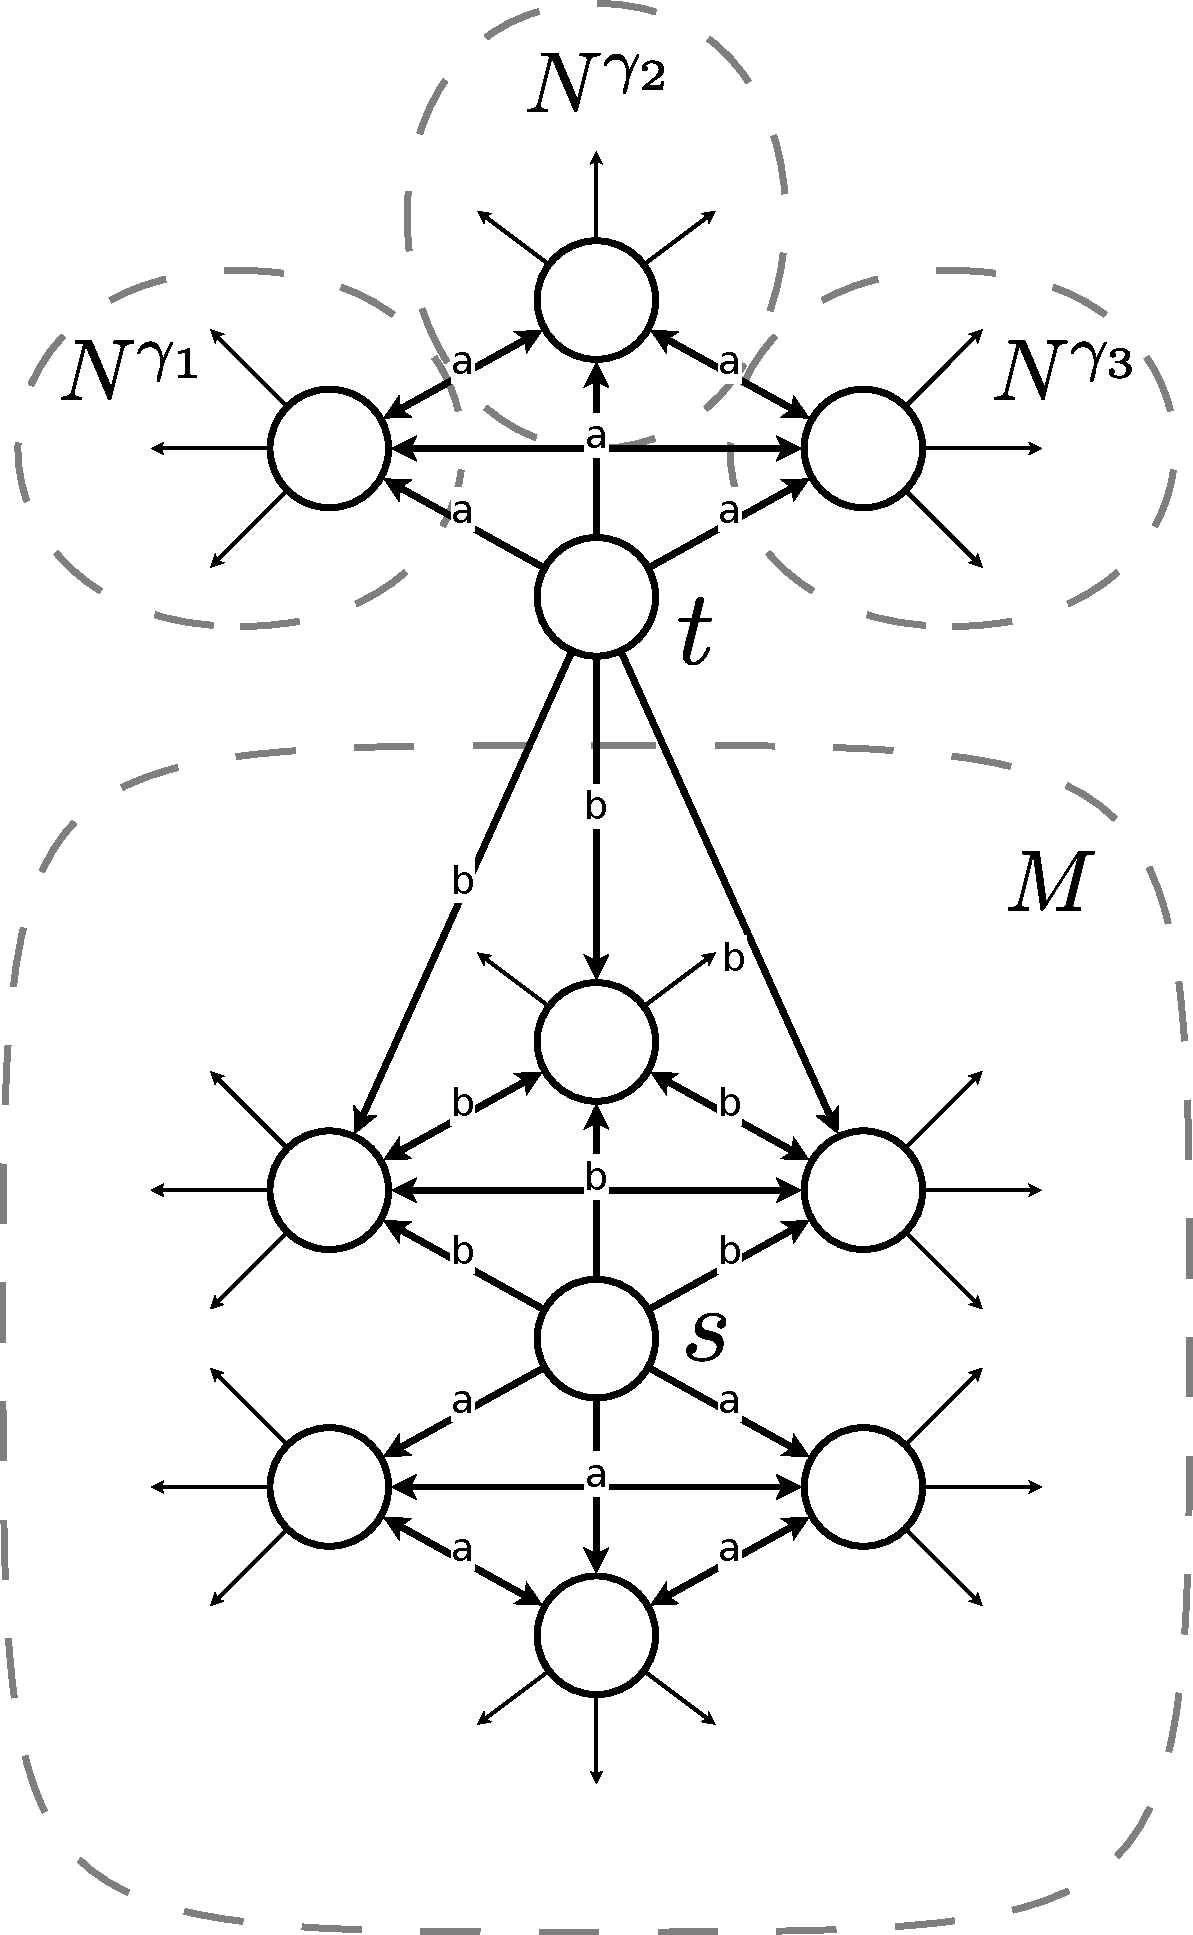
\includegraphics{rkd45}
}
\caption{
The model $N$ is constructed by taking the model $M$ and the models $N^\gamma$
for every $\gamma \in \Gamma_a$, and connecting them with an extra node $t$. $t$
is connected via an $a$-edge to $t^\gamma$ from each of the $N^\gamma$, and is
also connected via a $b$-edge to each $b$-successor of $s$ in $M$. We must also
have $a$-edges between each of the $t^\gamma$ to ensure that the resulting model
is transitive and Euclidean.
}
\end{center}
\end{figure}

We show that $N$ is a doxastic model. We must show two cases: that $R^N_a$
is serial, transitive and Euclidean, and that $R^N_b$ is also serial, transitive
and Euclidean, for every $b \in A - \{a\}$. As $M$ and each $N^\gamma$ are doxastic
models, the relations $R^M_c$ and $R^{N^\gamma}_c$ are serial, transitive and
Euclidean, for every $c \in A$. We observe that $S^N$ is a union of $\{t\}$,
$S^M$ and each $S^{N^\gamma}$. As $\Gamma_a$ is non-empty there is at
least one relationship $(t, t^\gamma)$ in $R^N_a$, therefore as $R^N_a$ also
contains $R^M_a$ and each $R^{N^\gamma}_a$, each of which are serial, then $R^N_a$
is also serial. Similarly, as $M$ is serial, $sR^M_b$ is non-empty, and so there
is at least one relationship $(t, t')$ where $t' \in sR^M_b$ in $R^N_b$;
therefore as $R^N_b$ also contains $R^M_b$ and $R^{N^\gamma}_b$, then $R^N_b$ is
also serial. To show the transitivity and Euclideaness of $R^N_a$, we first
observe that the relation can be considered in three independent parts; the
relationships between $t$ and $t^\gamma$, and between each $t^\gamma$; the
relation $R^M_a$; and the relations $R^{N^\gamma}_a$. The relation $R^M_a$ is
disjoint from the other relations, and so can be considered in isolation. By
hypothesis we have assumed that $t^\gamma R^{N^\gamma}_a = \{t^\gamma\}$, so as
there are no relationships from any $t^\gamma$ to a different state in
$S^{N^\gamma}$, we can also consider the each $R^{N^\gamma}_a$ separately from
the rest of $R^N_a$. We note that as $R^M_a$ and each $R^{N^\gamma}_a$ are
transitive and Euclidean, and as the remainder of the relation is essentially an
equivalence relation without the relationship $(t, t)$, it also has transitivity
and Euclideaness. Therefore $R^N_a$ is transitive and Euclidean. We can show
that $R^N_b$ is also transitive and Euclidean from the fact that $R^M_b$ and
each $R^{N^\gamma}_b$ is transitive and Euclidean, and otherwise disjoint from
each other, and the remainder of $R^N_b$ is simply a duplicate of relationships
from $s$ to its successors, then $R^N_b$ is also transitive and Euclidean.
Therefore $N$ is a doxastic model.

We construct an $a$-simulation $\mathcal{R}$ from $N_t$ to $M_s$, where:
$$\mathcal{R} = \{(t, s)\} \cup \{(s', s') \mid s' \in S^M \} 
\cup \bigcup_{\gamma \in \Gamma_a} \mathcal{R}^\gamma$$

We must show that $\mathcal{R}$ satisfies {\bf atoms}, {\bf forth-$b$} for every
$b \in A$, and {\bf back-$b$} for every $b \in A - \{a\}$.

\paragraph{atoms} We note that, by construction, the valuation of $N$ matches
the valuation of its corresponding states in $M$ and each $N^\gamma$, and the
valuation of $N_t$ matches that of $M_s$. Therefore $\mathcal{R}$ satisfies {\bf
atoms}.

\paragraph{forth} We next show that $\mathcal{R}$ satisfies {\bf forth-$b$} for
every $b \in A$.  Let $b \in A$ and let $(u, v) \in \mathcal{R}$.

Suppose that $(u, v) \in \mathcal{R}^\gamma$ for some $\gamma \in \Gamma_a$.
Suppose further that $b = a$ and $u = t^\gamma$ for some $\gamma \in \Gamma_a$.
Then $t^\gamma R^N_a = tR^N_a = \{t^{\gamma'} \mid \gamma' \in \Gamma_a\}$.  As
$M$ is a doxastic model, we have that $s^\gamma R^M_a = sR^M_a = \{s^{\gamma'}
\mid \gamma' \in \Gamma_a\}$, and as each $\mathcal{R}^{\gamma'}$ is an
$a$-simulation between $N^{\gamma'}_{t^{\gamma'}}$ and $M_{s^{\gamma'}}$, we
have that for every $\gamma' \in \Gamma_a$, $(t^{\gamma'}, s^{\gamma'}) \in
\mathcal{R}^{\gamma'} \subseteq \mathcal{R}$. Otherwise consider any other $(u,
v) \in \mathcal{R}^\gamma$.  Then as $\mathcal{R}^\gamma$ is an $a$-simulation,
it satisfies {\bf forth-$b$} for every $b \in A$. Hence for every $u' \in
uR^{N^\gamma}_b$, there exists some $v' \in vR^M_b$ such that $(u', v') \in
\mathcal{R}^\gamma \subseteq \mathcal{R}$. Suppose that $b = a$ and $u =
t^\gamma$ for some $\gamma \in \Gamma_a$.  

Suppose instead that $(u, v) = (s', s')$ for some $s' \in S^M$.  Then we note
that $s'R^N_b = s'R^M_b$, and hence for every $s'' \in s'R^N_b$ we have that
$s'' \in s'R^M_b$, and that $(s'', s'') \in \mathcal{R}$. 

Finally suppose that $(u, u') = (t, s)$. Then suppose that $b = a$. By
construction, $tR^N_a = \{t^\gamma \mid \gamma \in \Gamma_a\}$, and hence $v =
t^\gamma$ for some $\gamma \in \Gamma_a$. Hence we can take $s^\gamma \in
sR^M_a$, and note that as $\mathcal{R}^\gamma$ is an $a$-simulation from
$M_{s^\gamma}$ to $N^\gamma_{t^\gamma}$, we know that $(t^\gamma, s^\gamma) \in
\mathcal{R}^\gamma \subseteq \mathcal{R}$. Suppose that $b \neq a$. Then by
construction, $tR^M_b = sR^M_b$, hence for every $t' \in tR^M_b$, we have that
$t' \in sR^M_b$, and hence we know that $(t', t') \in \mathcal{R}$. Hence
$\mathcal{R}$ satisfies {\bf back-$b$} for every $b \in A$.  matches that of
$M_s$. Therefore $\mathcal{R}$ satisfies {\bf atoms}.

\paragraph{back} A similar argument to above shows that $\mathcal{R}$ satisfies
{\bf back-$b$} for every $b \in A - \{a\}$.

Therefore $\mathcal{R}$ is an $a$-simulation, and $N_t \refinement_a M_s$. 

Finally we show that $N_t \entails \covers_a \Gamma_a$. We must show that for
each $\gamma \in \Gamma_a$ that $N_{t^\gamma} \entails \gamma$. As each $\gamma$
is an $a$-disjunctive normal formula, a similar argument to that used in
Lemma~\ref{kd45-successors} can be used to show that each of the successors of
$N_{t^\gamma}$ are bisimilar to the corresponding successors of
$N^\gamma_{t^\gamma}$. This is obvious, as $N$ contains a duplicate of
$N^\gamma$, and $N$ does not contain any additional edges originating from
states in $S^{N^\gamma}$, except for $a$-edges from $t^\gamma$. Hence we have
that $N_{t^\gamma} \entails \gamma$ for every $\gamma \in \Gamma_a$, and hence
$N_t \entails \covers_a \Gamma$.

As $N_t \refinement_a M_s$, and $N_t \entails \covers_a \Gamma_a$ we therefore
have that $M_s \entails \somerefs_a \covers_a \Gamma_a$.

Conversely, suppose that $M_s \entails \covers_a \Gamma_a$. Then there exists a
doxastic model $N_t \refinement_a M_s$, via some $a$-simulation $\mathcal{R}$,
such that $N_t \entails \covers_a \Gamma_a$. From the definition of the cover
operator, this implies that $N_t \entails \knows_a \bigvee_{\gamma \in \Gamma_a}
\gamma \land \bigwedge_{\gamma \in \Gamma_a} \suspects_a \gamma$. In particular we
note that for every $\gamma \in \Gamma_a$, $N_t \entails \suspects_a \gamma$, and
so there exists some $t^\gamma \in tR^N_a$ such that $N_{t^\gamma} \entails
\gamma$. As $t^\gamma \in tR^N_a$, and $(t, s) \in \mathcal{R}$, by {\bf
forth-$a$} there exists some $s^\gamma \in sR^M_a$ such that $(t^\gamma, s^\gamma)
\in \mathcal{R}$. Hence $\mathcal{R}$ is also an $a$-simulation from
$N_{t^\gamma}$ to $M_{s^\gamma}$, and so $M_{s^\gamma} \entails \somerefs_a
\gamma$. As for every $\gamma \in \Gamma_a$ we have that $s^\gamma \in sR^M_a$, we
also have that $M_s \entails \suspects_a \somerefs_a \gamma$. Therefore we
finally have that $M_s \entails \bigwedge_{\gamma \in \Gamma_a} \suspects_a
\somerefs_a \gamma$.

Therefore {\bf RKD45} is sound.

\paragraph{RComm} 
Suppose that $M_s \in \classKD$ is a doxastic model such that $M_s \entails
\covers_b \{ \somerefs_a \gamma \mid \gamma \in \Gamma_b\}$, where $a \ne b$ and
$\Gamma_b$ is a non-empty set of $b$-disjunctive normal formulae. 

We need to show that $M_s \entails \somerefs_a \covers_b \Gamma_b$. To do this
we follow the same strategy as for proving {\bf RKD45}: we construct an
$a$-refinement $N_t \in \classKD$, and show that $N_t \entails \covers_b
\Gamma$.

We begin by constructing the model $N_t$. Consider $\gamma \in \Gamma$. From
$M_s \entails \covers_b \{ \somerefs_a \gamma \mid \gamma \in \Gamma_b\}$, there
exists a state $s^\gamma \in sR^M_b$ such that $M_{s^\gamma} \entails
\somerefs_a \gamma$. Therefore there exists a doxastic model
$N^\gamma_{t^\gamma} \refinement_a M_{s^\gamma}$, via some $a$-simulation
$\mathcal{R}^\gamma$, such that $N^\gamma_{t^\gamma} \entails \gamma$.  Without
loss of generality we assume that the $N^\gamma$ are disjoint. We may also
assume, by Lemma~\ref{kd45-successors}, that for every $\gamma \in \Gamma$,
$t^\gamma R^{N^\gamma}_b = R^{N^\gamma}_b t^\gamma = \{t^\gamma\}$ and that
$R^{N^\gamma}_c t^\gamma = \emptyset$ for every $c \in A - \{b\}$.

Let $t$ be a state not in $S^M$ or any of the $S^{N^\gamma}$. Then we construct
a Kripke model $N = (S^N, R^N, V^N)$ where:
\begin{eqnarray*}
S^N &=& \{t\} \cup S^M \bigcup_{\gamma \in \Gamma_b} S^{N^\gamma}\\
R^N_b &=& \{(t, t^\gamma) \mid \gamma \in \Gamma_b\} \cup \{(t^\gamma,
t^{\gamma'}) \mid \gamma, \gamma' \in \Gamma_b\} \cup R^M_b \cup \bigcup_{\gamma
\in \Gamma_b} R^{N^\gamma}_b\\
R^N_c &=& \{(t, t') \mid t' \in sR^M_c\} \cup R^M_c \cup \bigcup_{\gamma \in
\Gamma_b} R^{N^\gamma}_c \text{ for $c \in A - \{b\}$}\\
V^N(p) &=& 
\begin{cases}
\displaystyle \{t\} \cup V^M(p) \cup \bigcup_{\gamma \in \Gamma_b}
V^{N^\gamma}(p) & \text{if $s \in V^M(p)$}\\
\displaystyle V^M(p) \cup \bigcup_{\gamma \in \Gamma_b} V^{N^\gamma}(p) &
\text{otherwise}
\end{cases}
\text{ for $p \in P$}
\end{eqnarray*}

We note that $N$ is a doxastic model, by similar arguments as used in the proof
for {\bf RKD45}.

We construct an $a$-simulation $\mathcal{R}$ from $N_t$ to $M_s$, where:
$$\mathcal{R} = \{(t, s)\} \cup \{(s', s') \mid s' \in S^M\} \cup \bigcup_{\gamma \in \Gamma_b} \mathcal{R}^\gamma$$

We note that $\mathcal{R}$ is an $a$-simulation, by similar arguments as used in
the proof for {\bf RKD45}. In particular, this means that $N_t \refinement_a
M_s$.

We also note that for every $\gamma \in \Gamma_b$, that $N_{t^\gamma} \entails
\gamma$, by similar arguments as used in the proof for {\bf RKD45}. In
particular, this means that $N^\gamma_t \entails \covers_b \Gamma_b$.

Therefore $M_s \entails \somerefs_a \covers_b \Gamma_b$.

The converse, $\somerefs_a \covers_b \Gamma_b \implies \covers_b \{\somerefs_a
\gamma \mid \gamma \in \Gamma_b\}$ follows a similar proof to the relevant part in
the proof for {\bf RKD45}.

Therefore {\bf RComm} is sound.

\paragraph{RDist} 
Suppose that $M_s$ is a doxastic model such that $M_s \entails \bigwedge_{b \in
B} \somerefs_a \covers_b \Gamma_b$, where $B \subseteq A$, and $\Gamma_b$ is a
set of $b$-disjunctive formulae for each $b \in B$.

We need to show that $M_s \entails \somerefs_a \bigwedge_{b \in B} \covers_b
\Gamma_b$. To do this we follow the same strategy as for proving {\bf RKD45}: we
construct an $a$-refinement $N_t \in \classKD$, and show that $N_t \entails
\somerefs_a \bigwedge_{b \in B} \covers_b \Gamma_b$.

We begin by constructing the model $N_t$. Suppose that $a \in B$. Then we have
$M_s \entails \somerefs_a \covers_a \Gamma_a$, and by {\bf RKD45} this implies that
$M_s \entails \bigwedge_{\gamma \in \Gamma_a} \gamma$. We also have that for
every $b \in B - \{a\}$ that $M_s \entails \somerefs_a \covers_a \Gamma_b$, and
by {\bf RComm} this implies that $M_s \entails \covers_b \{\somerefs_a \gamma
\mid \gamma \in \Gamma_b\}$, and by the definition of the cover operator, this
implies that $M_s \entails \bigwedge_{\gamma \in \Gamma_b} \suspects_b
\somerefs_a \gamma$. Hence for every $b \in B$ and $\gamma \in \Gamma_b$, we
have that $\suspects_b \somerefs_a \gamma$. This implies that for each $b \in B$
and each $\gamma \in \Gamma_b$ that there exists some $s^{b,\gamma} \in sR^M_b$ such
that $M_{s^{a,\gamma}} \entails \somerefs_a \gamma$. Therefore there exists a
doxastic model $N^{b,\gamma}_{t^{b,\gamma}} \refinement_a M_{s^{a,\gamma}}$ such
that $N^{b,\gamma}_{t^{b,\gamma}} \entails \gamma$. Without loss of generality
we may assume that the $N^{b,\gamma}$ are disjoint. We may also assume, by
Lemma~\ref{kd45-successors}, that for every $b \in B$ and $\gamma \in \Gamma$,
that $t^\gamma R^{N^\gamma}_b = R^{N^\gamma}_b t^\gamma = \{t^\gamma\}$ and that
$R^{N^\gamma}_c t^\gamma = \emptyset$ for every $c \in A - \{b\}$.

Let $t$ be a state not in $S^M$ or any of the $S^{N^{b,\gamma}}$. Then we
construct a Kripke model $N = (S^N, R^N, V^N)$ where:
\begin{eqnarray*}
S^N &=& \{t\} \cup \bigcup_{b \in A, \gamma \in \Gamma_b} S^{N^{b,\gamma}}\\
R^N_b &=& \{(t, t^{b,\gamma}) \mid b \in A, \gamma \in \Gamma_b\} 
\cup \{(t^{b,\gamma}, t^{b,\gamma'}) \mid \gamma, \gamma' \in \Gamma_b\}\\
&&\qquad \cup \bigcup_{c \in A, \gamma \in \Gamma_b} R^{N^{c,\gamma}}_b \text{ for $b \in A$}\\
R^N_b &=& \{(t, t') \mid t' \in sR^M_b\} \cup R^M_b \cup
\bigcup_{c \in B, \gamma \in \Gamma_c} R^{N^{c,\gamma}}_b \text{ for $b \in A
\setminus B$}\\
V^N(p) &=& 
\begin{cases}
\displaystyle \{t\} \cup \bigcup_{b \in A, \gamma \in \Gamma_b} V^{N^{b,\gamma}}(p)
& \text{if $s \in V^M(p)$}\\
\displaystyle \bigcup_{b \in A, \gamma \in \Gamma_b} V^{N^{b,\gamma}}(p) &
\text{otherwise}
\end{cases}
\end{eqnarray*}

We note that $N$ is a doxastic model, by similar arguments as used in the proof
for {\bf RKD45}.

We construct an $a$-simulation $\mathcal{R}$ from $N_t$ to $M_s$, where:
$$\mathcal{R} = \{(t, s)\} \cup \bigcup_{b \in A, \gamma \in \Gamma_b}
\mathcal{R}^\gamma$$

We note that this is an $a$-simulation, by similar arguments as used in the
proof for {\bf RKD45}. In particular, this means that $N_t \refinement_a M_s$.

We also note that for every $\gamma \in \Gamma_b$, that $N_{t^\gamma} \entails
\gamma$, by similar arguments as used in the proof for {\bf RKD45}. In
particular, this means that $N^\gamma_t \entails \covers_b \Gamma_b$.

Therefore $M_s \entails \somerefs_a \bigwedge_{b \in A} \covers_b \Gamma_b$ and
{\bf RDist} is sound.

Therefore the axiomatisation \axiomKDF{} is sound.
\end{proof}

We note that, similar to \axiomKF{}, the converse of {\bf RDist} is derivable
within \axiomKDF{}.

\begin{lemma}\label{kd45-rdist-converse}
The following is derivable in \axiomKDF{}.
$$
\proves \bigwedge_{b \in A} \somerefs_a \covers_b \Gamma_b \iff
\somerefs_a \bigwedge_{b \in A} \covers_b \Gamma_b \\
$$
where $\Gamma_b$ is a set of $b$-disjunctive normal formulae for
every $b \in A$.
\end{lemma}

We show the completeness of the axiomatisation \axiomKDF{} in a similar fashion
to the completeness proof of \axiomKF{}, by a provably correct translation from
\langF{} to \lang{}. Completeness then follows from the completeness of
\logicKD{}.

As for the completeness proof for \axiomKF{}, we introduce some similar
equivalences that will be used by our translation.

\begin{lemma}\label{kd45-equivalences}
The following are provable equivalences using \axiomKDF{}:
\begin{enumerate}
\item $\displaystyle \somerefs_a (\phi \lor \psi) \iff
\somerefs_a \phi \lor \somerefs_a \psi$
\item $\displaystyle \somerefs_a (\pi \land \bigwedge_{b
\in B} \covers_b \Gamma_b) \iff \pi \land \bigwedge_{\gamma \in \Gamma_a}
\suspects_a \somerefs_a \gamma \land \bigwedge_{b \in B} \covers_b \{\somerefs_a
\gamma \mid \gamma \in \Gamma_b\}$ where $\pi$ is propositional, $B \subseteq
A$, and $a \in B$
\item $\displaystyle \somerefs_a (\pi \land \bigwedge_{b
\in B} \covers_b \Gamma_b) \iff \pi \land \bigwedge_{b \in B} \covers_b
\{\somerefs_a \gamma \mid \gamma \in \Gamma_b\}$ where $\pi$ is propositional,
$B \subseteq A$, and $a \notin B$
\end{enumerate}
where for every $a \in A$, the set $\Gamma_a$ is a non-empty set of
$a$-disjunctive normal formulae.
\end{lemma}

This can be shown by following similar reasoning as used for the proof of
Lemma~\ref{k-equivalences}, but by substituting \axiomKF{} axioms for
\axiomKDF{} axioms.

\begin{lemma}\label{kd45-translation}
Every formula of \logicKDF{} is provably equivalent to a formula of \logicKD{}.
\end{lemma}

This can be shown following similar reasoning as used for the proof of
Lemma~\ref{k-translation}. We note that, of course, we use the appropriate
axioms of \axiomKDF{} in place of those from \axiomKF{}, and we also use the
equivalences from Lemma~\ref{kd45-equivalences} in place of those from
Lemma~\ref{k-equivalences}. We also use the assumption that formulae are in
the doxastic version of cover logic disjunctive normal form, rather than the
modal version of disjunctive normal form.

The rest of the completeness proof follows the same reasoning as used for the
completeness proof of \axiomKF{}.

\begin{corollary}\label{kd45-derivable}
Let $\phi \in \logicKDF$ be given and $\psi \in \logicKD$ be semantically
equivalent to $\phi$.  If $\psi$ is a theorem in \logicKD{}, then $\phi$ is a
theorem in \axiomKDF{}.
\end{corollary}

\begin{lemma}\label{kd45-complete}
The axiom schema \axiomKDF{} is complete with respect to the semantic class
\classKD{}.
\end{lemma}

We note that Corollary~\ref{kd45-derivable} and Lemma~\ref{kd45-complete} can be
shown by following similar reasoning as used for the proofs of
Corollary~\ref{k-derivable} and Lemma~\ref{k-complete} respectively.

\begin{theorem}
The axiomatisation \axiomKDF{} is sound and complete with respect to the
semantic class \classKD{}.
\end{theorem}

\begin{proof}
The soundness proof is given in Lemma~\ref{kd45-sound} and the completeness
proof is given in Lemma~\ref{kd45-complete}.
\end{proof}

We note that, as in the axiomatisation for the single-agent epistemic and
doxastic logics, the completeness proofs above were performed with a provably
correct translation from \langF{} to \lang{}, under the semantics of
\logicKDF{}. This shows that \logicKDF{} is expressively equivalent to
\logicKD{}, and allows us to show several results. In particular, \logicKDF{} is
decidable.

\begin{theorem}
The logic \logicKDF{} is decidable.
\end{theorem}

This can be shown by following similar reasoning as used for the proof of
Theorem~\ref{single-decidable}.
